% *********************************************************************
% © 2021-2023 Jeremy Sylvestre
%
% Permission is granted to copy, distribute and/or modify this document
% under the terms of the GNU Free Documentation License, Version 1.3 or
% any later version published by the Free Software Foundation; with no
% Invariant Sections, no Front-Cover Texts, and no Back-Cover Texts. A
% copy of the license is included in the appendix entitled “GNU Free
% Documentation License” that appears in the output document of this
% PreTeXt source code. All trademarks™ are the registered® marks of
% their respective owners.
%
% *********************************************************************

\newcommand*{\xmin}{0}
\newcommand*{\xmax}{6}
\newcommand*{\ymin}{-3}
\newcommand*{\ymax}{18}

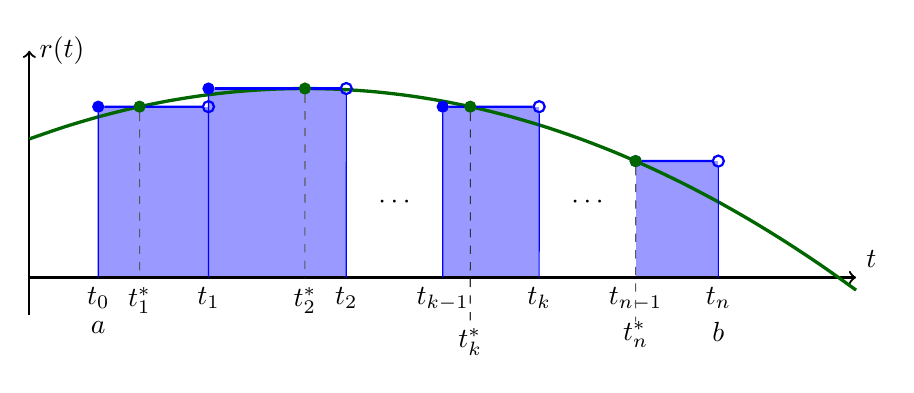
\begin{tikzpicture}
[
	closedpt/.style={circle,draw,fill,inner sep=0pt,minimum size=4pt},
	openpt/.style={circle,draw,inner sep=0pt,minimum size=4pt},
	xscale=1.75,
	yscale=0.16
]

	% rectangle fills
	\fill[blue!40!white] (0.5,13.56) rectangle (1.3,0);
	\fill[blue!40!white] (1.3,15) rectangle (2.3,0);
	\fill[blue!40!white] (3,13.56) rectangle (3.7,0);
	\fill[blue!40!white] (4.4,9.24) rectangle (5,0);

	% labels
	\node[below] at (0.5,0) {$t_0$};
	\node[below,yshift=-12.5] at (0.5,0) {$a$};
	\node[below] at (5,0) {$t_n$};
	\node[below,yshift=-12.5] at (5,0) {$b$};

	\node[below] at (0.8,0) {$t_1^\ast$};
	\node[below] at (1.3,0) {$t_1$};

	\node[below] at (2,0) {$t_2^\ast$};
	\node[below] at (2.3,0) {$t_2$};

	\node at (2.65,6) {$\cdots$};

	\node[below] at (3,0) {$t_{k-1}$};
	\node[below,yshift=-15] at (3.2,0) {$t_k^\ast$};
	\node[below] at (3.7,0) {$t_k$};

	\node at (4.05,6) {$\cdots$};

	\node[below] at (4.4,0) {$t_{n-1}$};
	\node[below,yshift=-12.5] at (4.4,0) {$t_n^\ast$};

	% axes
	\draw[->,thick] (\xmin,0) -- (\xmax,0) node[above right] {$t$};
	\draw[->,thick] (0,\ymin) -- (0,\ymax) node[right] {$r(t)$};

	% continuous graph
	\draw[green!40!black,very thick,domain=0:6,smooth] plot (\x,{- \x * \x + 4 * \x + 11});

	% levels and dividers

	\node[blue,closedpt] at (0.5,13.56) (start) {};
	\draw[blue,thin] (start) -- (0.5,0);
	\node[blue,thick,openpt] at (1.3,13.56) (stop) {};
	\draw[blue,thick] (start) -- (stop);
	\node[green!40!black,closedpt] at (0.8,13.56) (sample) {};
	\draw[black!65!white,dashed] (sample) -- (0.8,0);

	\node[blue,closedpt] at (1.3,15) (start) {};
	\draw[blue,thin]
	  (stop) -- (start)
	  (start) -- (1.3,0)
	;
	\node[blue,thick,openpt] at (2.3,15) (stop) {};
	\draw[blue,thick] (start) -- (stop);
	\draw[blue,thin] (stop) -- (2.3,0);
	\node[green!40!black,closedpt] at (2,15) (sample) {};
	\draw[black!65!white,dashed] (sample) -- (2,0);

	\node[blue,closedpt] at (3,13.56) (start) {};
	\node[blue,thick,openpt] at (3.7,13.56) (stop) {};
	\draw[blue,thick] (start) -- (stop);
	\draw[blue,thin]
	  (start) -- (3,0)
	  (stop) -- (3.7,0)
	;
	\node[green!40!black,closedpt] at (3.2,13.56) (sample) {};
	\draw[black!80!white,dashed] (sample) -- (3.2,-3.5);

	\node[blue,closedpt] at (4.4,9.24) (start) {};
	\node[blue,thick,openpt] at (5,9.24) (stop) {};
	\draw[blue,thick] (start) -- (stop);
	\draw[blue,thin] (stop) -- (5,0);
	\node[green!40!black,closedpt] at (4.4,9.24) (sample) {};
	\draw[black!65!white,dashed] (sample) -- (4.4,-3.5);

\end{tikzpicture}
